\documentclass[a4paper]{article}
\usepackage{fancyhdr}
\usepackage[pdftex]{graphicx}
\usepackage{sidecap}
\usepackage{listings}
\usepackage{color}
\usepackage[export]{adjustbox}
\usepackage{subcaption}

\usepackage{hyperref}
\hypersetup{
    colorlinks=true,
    linkcolor=blue,
    filecolor=magenta, 
    urlcolor=cyan,
    bookmarks=true,
    pdfpagemode=FullScreen,
}
\usepackage{geometry}
 \geometry{
 a4paper,
 total={210mm,297mm},
 left=15mm,
 right=15mm,
 top=15mm,
 bottom=15mm,
 }

\usepackage{glossaries}


\makeglossaries
\newglossaryentry{FSM}
{
    name=FSM,
    description={Finite State Machine}
}

\definecolor{mygreen}{RGB}{25,172,0} % color values Red, Green, Blue
\definecolor{mylilas}{RGB}{170,55,241}
\definecolor{dkgreen}{rgb}{0,0.6,0}
\definecolor{gray}{rgb}{0.5,0.5,0.5}
\definecolor{mauve}{rgb}{0.58,0,0.82}

\pagestyle{fancy}
\fancyhf{}
\rhead{Vangjush Komini}
\lhead{KU Leuven}
\rfoot{Page \thepage}
\lfoot{Biomedical Data Processing part 2}


\lstset{inputpath=Code2}
\graphicspath{{Images2/}}

\include{Glossary}


\begin{titlepage}

\title{Assignment2\\\centerline{\textit{Nonlinear signal processing}} }

\author{
\href{mailto:vangjush.komini@uzleuven.be}{Vangjush Komini}\\  \textit{r0612470} \\
\href{mailto:vangjush.komini@uzleuven.be}{vangjush.komini@uzleuven.be}\\
}





\end{titlepage}




\begin{document}



\maketitle
\begin{center}
\Large \href{https://onderwijsaanbod.kuleuven.be/syllabi/e/H06W1AE.htm#activetab=doelstellingen_idp41200}{Biomedical Data Processing, Part II Course}
\end{center}

\begin{figure}[!htbp]
\centering

\includegraphics[width=0.4\textwidth]{icon1.png}
\end{figure}







\section{Artefact removal for EEG data}




\begin{figure}[!htbp]
\minipage{.5\textwidth}%
\centering
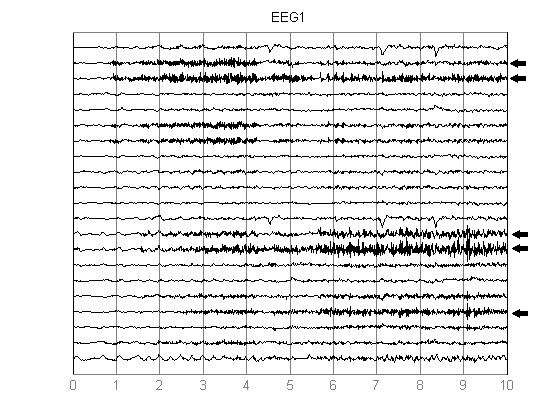
\includegraphics[width=.8\textwidth]{1.jpg}
\subcaption{EEG signal of the first set}
\endminipage\hfill
\minipage{.5\textwidth}%
\centering
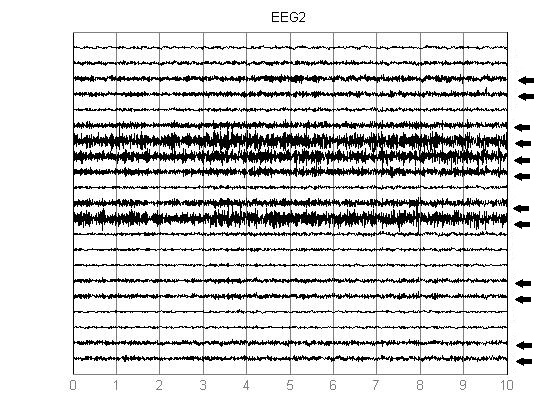
\includegraphics[width=.8\textwidth]{2.jpg}
\subcaption{EEG signal of the second set}
\endminipage\hfill
\caption{Orgininal EEG signals where in addition the most affected channels by the muscles artifacts are pointed out}
\end{figure}


\begin{figure}[!htbp]
\minipage{.3\textwidth}%
\centering
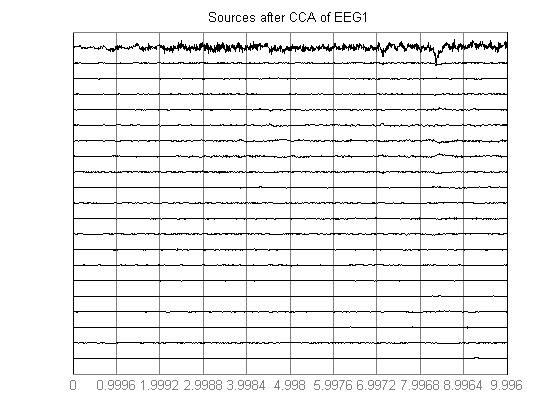
\includegraphics[width=1\textwidth]{3.jpg}
\subcaption{EEG reconstructed signals after CCA}
\endminipage\hfill
\minipage{.3\textwidth}%
\centering
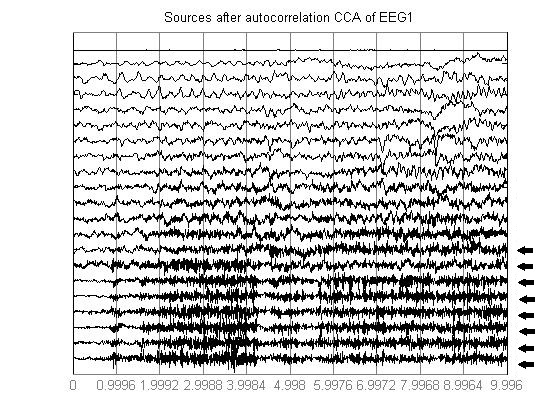
\includegraphics[width=1\textwidth]{4.jpg}
\subcaption{The CCA source channel}
\endminipage\hfill
\minipage{.3\textwidth}%
\centering
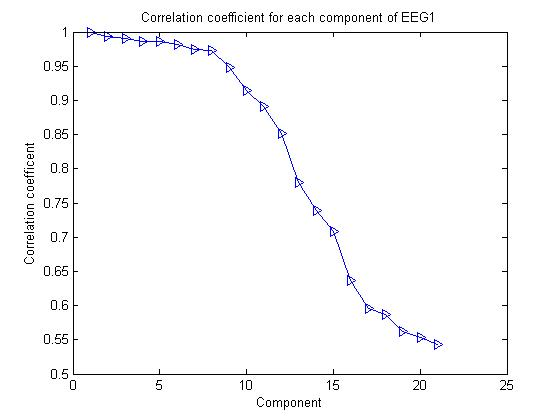
\includegraphics[width=1\textwidth]{5.jpg}
\subcaption{Correlation values for respective channel}
\endminipage\hfill
\caption{CCA outcome for the first data set}
\end{figure}

\begin{figure}[!htbp]
\minipage{.3\textwidth}%
\centering
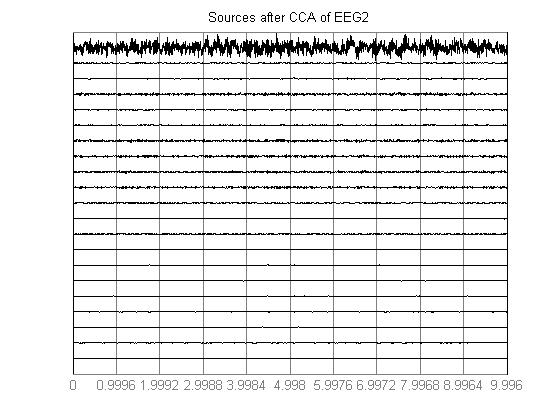
\includegraphics[width=1\textwidth]{6.jpg}
\subcaption{EEG reconstructed signals after CCA}
\endminipage\hfill
\minipage{.3\textwidth}%
\centering
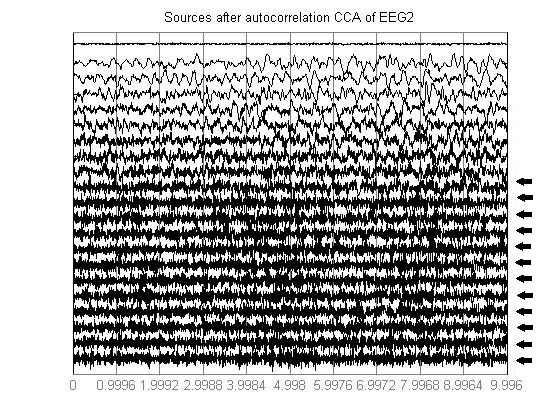
\includegraphics[width=1\textwidth]{7.jpg}
\subcaption{The CCA source channel}
\endminipage\hfill
\minipage{.3\textwidth}%
\centering
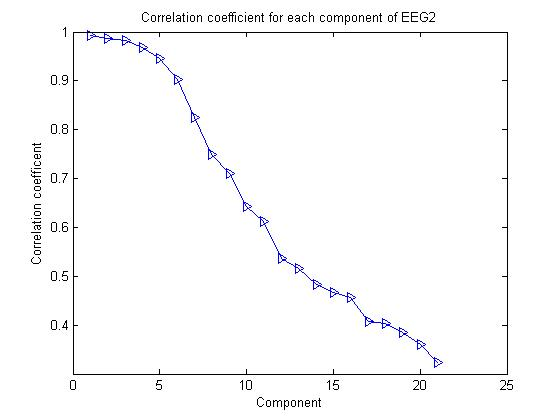
\includegraphics[width=1\textwidth]{8.jpg}
\subcaption{Correlation values for respective channel}
\endminipage\hfill
\caption{CCA outcome for the second data set}
\end{figure}

\begin{figure}[!htbp]
\minipage{.3\textwidth}%
\centering
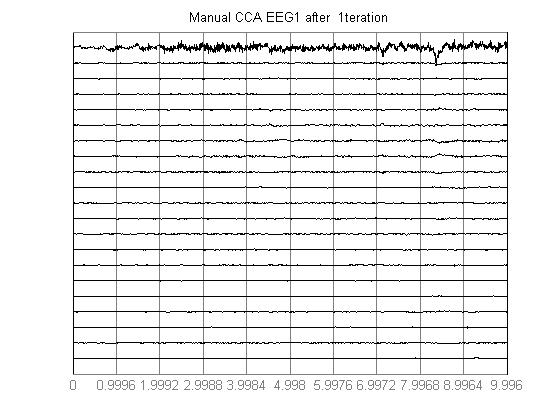
\includegraphics[width=1\textwidth]{9.jpg}\\
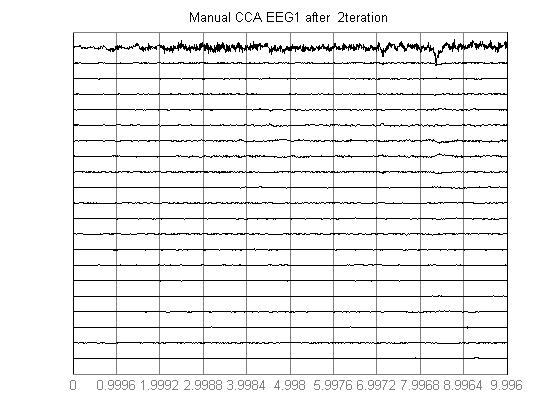
\includegraphics[width=1\textwidth]{10.jpg}
\endminipage\hfill
\minipage{.3\textwidth}%
\centering
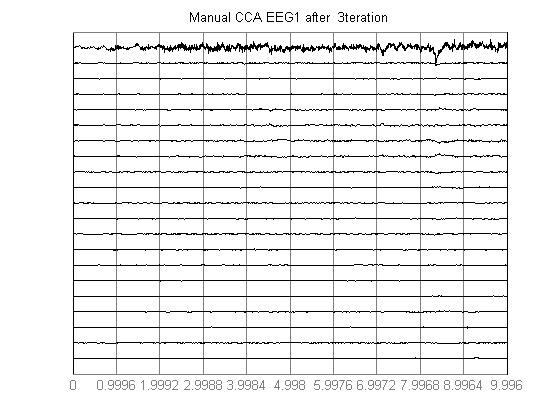
\includegraphics[width=1\textwidth]{11.jpg}\\
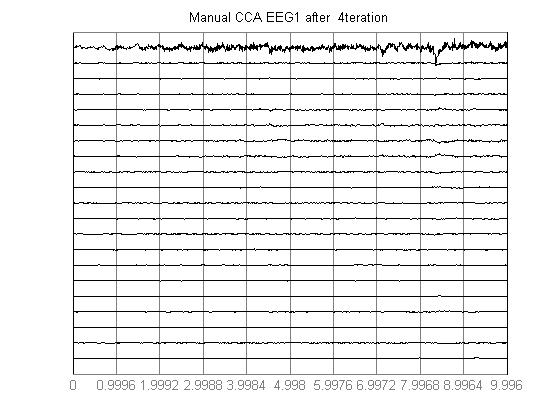
\includegraphics[width=1\textwidth]{12.jpg}
\endminipage\hfill
\minipage{.3\textwidth}%
\centering
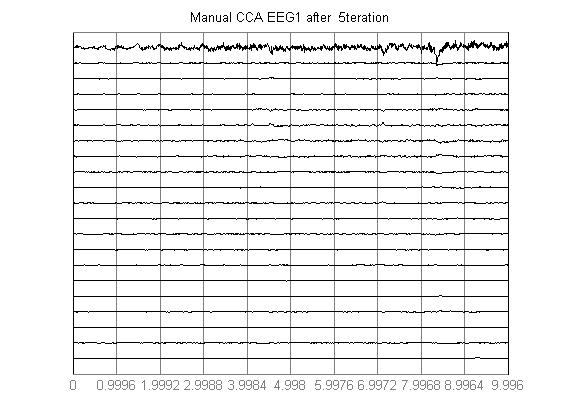
\includegraphics[width=1\textwidth]{13.jpg}\\
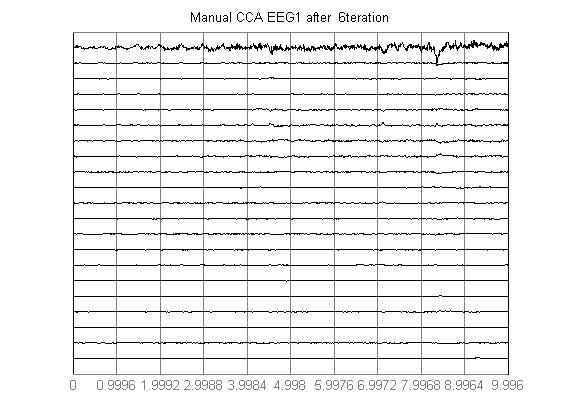
\includegraphics[width=1\textwidth]{14.jpg}
\endminipage\hfill
\caption{Manual CCA processing of the first EEG data set signal where the last plot outlines the noisy free EEG signal}\label{today4}
\end{figure}


\begin{figure}[!htbp]
\minipage{.3\textwidth}%
\centering
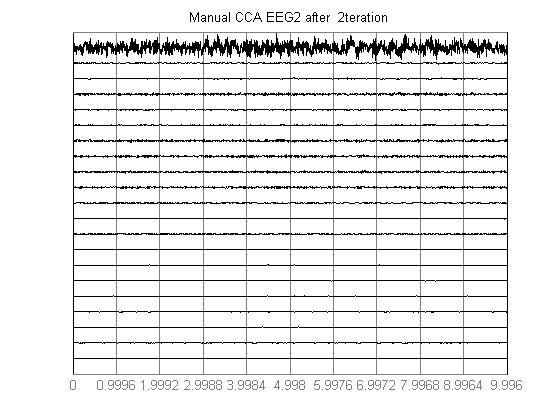
\includegraphics[width=1\textwidth]{16.jpg}\\
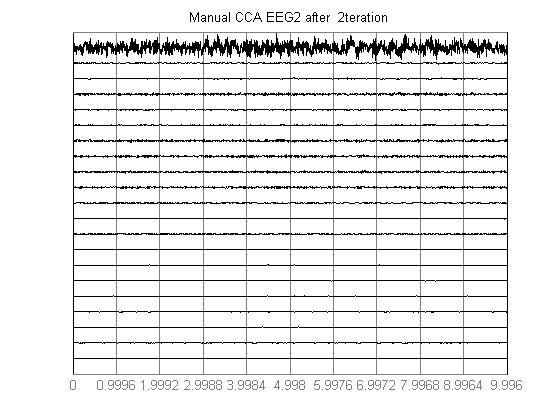
\includegraphics[width=1\textwidth]{16.jpg}\\
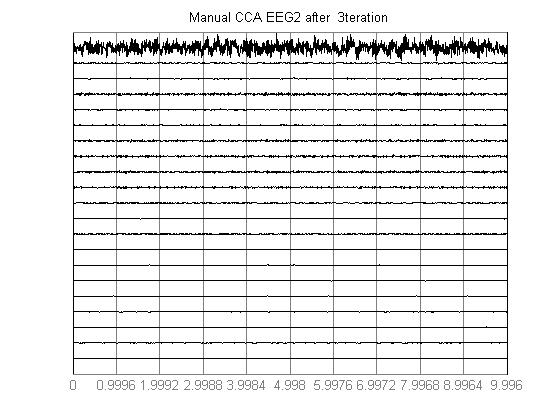
\includegraphics[width=1\textwidth]{17.jpg}\\
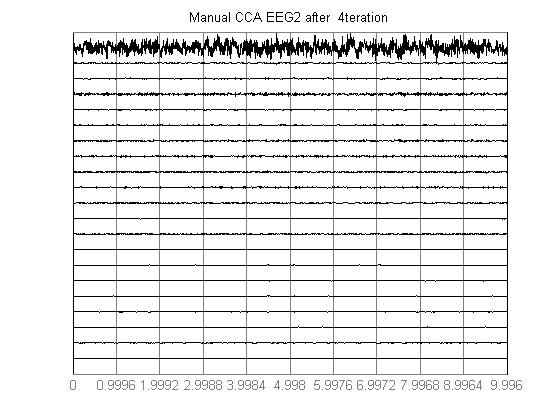
\includegraphics[width=1\textwidth]{18.jpg}
\endminipage\hfill
\minipage{.3\textwidth}%
\centering
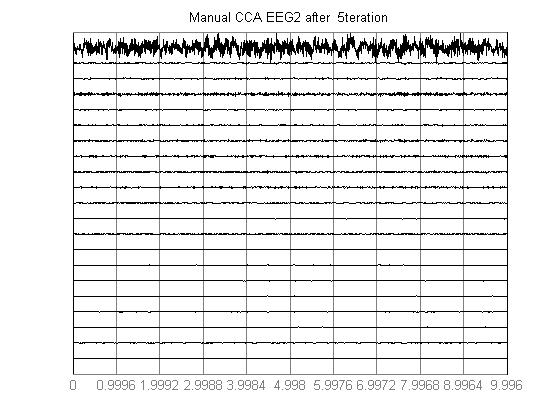
\includegraphics[width=1\textwidth]{19.jpg}\\
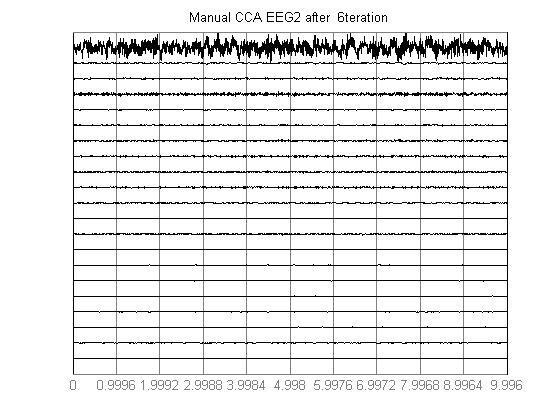
\includegraphics[width=1\textwidth]{20.jpg}\\
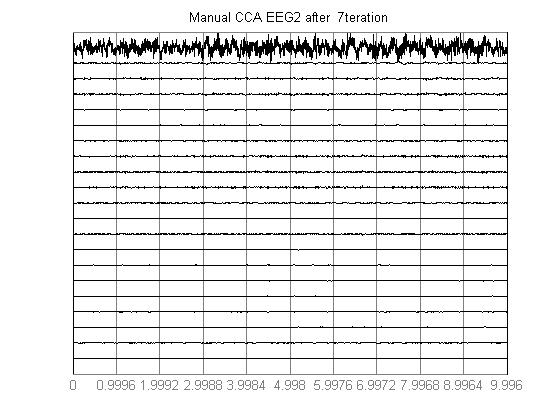
\includegraphics[width=1\textwidth]{21.jpg}\\
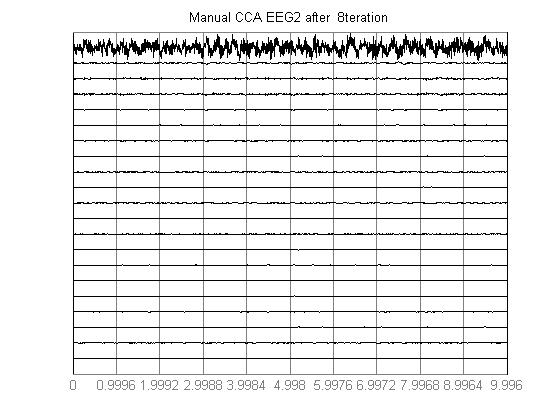
\includegraphics[width=1\textwidth]{22.jpg}
\endminipage\hfill
\minipage{.3\textwidth}%
\centering

\includegraphics[width=1\textwidth]{23.jpg}\\
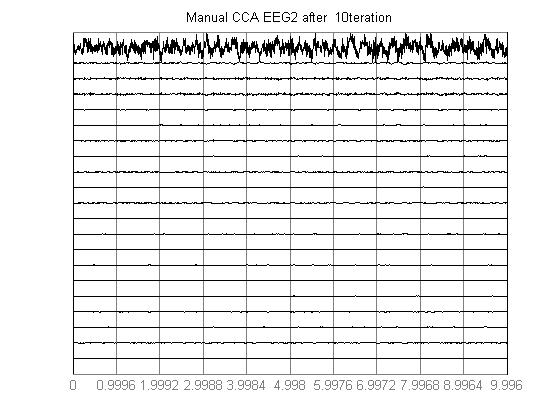
\includegraphics[width=1\textwidth]{24.jpg}\\
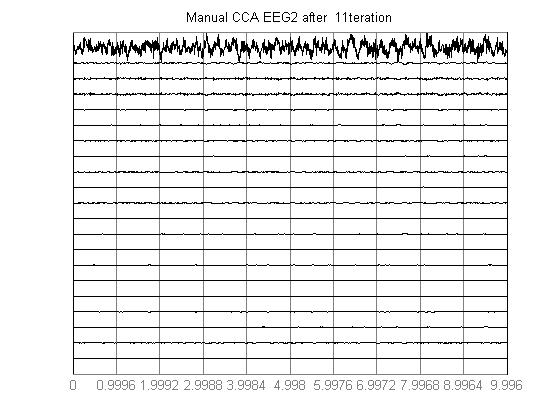
\includegraphics[width=1\textwidth]{25.jpg}\\
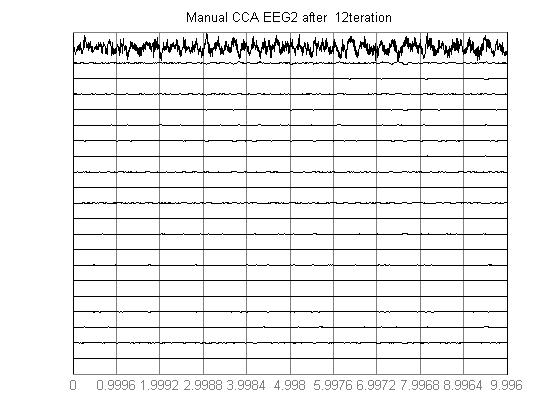
\includegraphics[width=1\textwidth]{26.jpg}
\endminipage\hfill
\caption{Manual CCA processing of the second EEG data set signal where the last plot outlines the noisy free EEG signal}\label{today3}
\end{figure}


\begin{figure}[!htbp]
\minipage{.5\textwidth}%
\centering
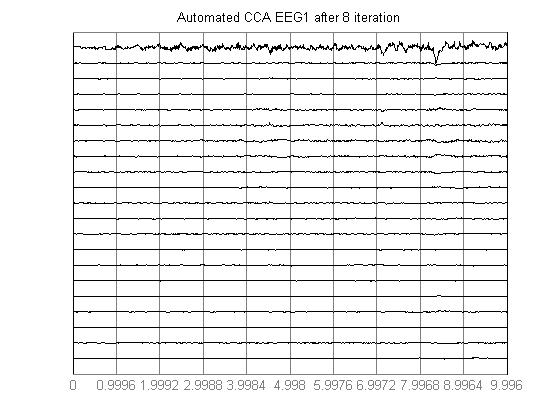
\includegraphics[width=1\textwidth]{27.jpg}
\subcaption{CCA results of the first data set}\label{toda1}
\endminipage\hfill
\minipage{.5\textwidth}%
\centering
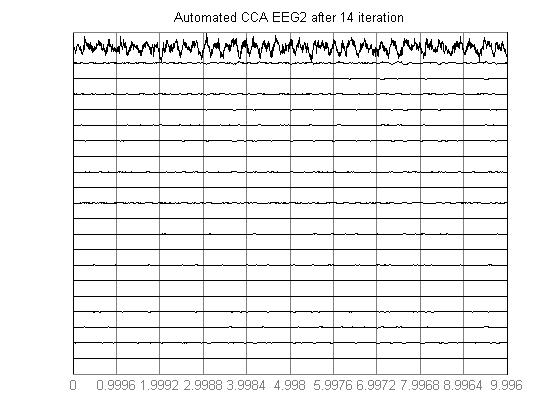
\includegraphics[width=1\textwidth]{28.jpg}
\subcaption{CCA results of the second data set}\label{toda2}
\endminipage\hfill
\caption{Automated processing of the CCA signals}
\end{figure}

CCA is very difficult to make it fully automated. Yet it is possible to make it semi automatic by erasing some of the channels where the correlation values is definitely without any influence into the signal. Moving into higher correlation values removing the channels manually increases the accuracy of the processing. Since this channels contain also information apart from the artifacts an accurate learning algorithm yet cannot decided precisely when to do this process. Nevertheless an automated method has been applied to remove the noisy signal by removing all those CCA channels where the correlation values is smaller than $0.7$. The results for this are outlined in the figure \ref{toda1} and \label{toda2} for the first and the second data set of the EEG signals. Whereas in the figure \ref{today3} and \ref{today4} are the manual results of the first and the second EEG data set. Furthermore the number of channels removed in the manual execution is much lower compare to the automatic case. This is the case because the visual classification is far better compare defining the the removed channel via the correlation coefficient.  

The two data set however contain different level of the artifact. The correlation coefficients for the first data set tends to sit into higher values compare to the second data set. Consequently the number of channels removed manually is much higher in the in the second data set. Even though the number of channels that are being removed are chosen manually, some  muscles artifact are hard to be removed via CCA. This is from the statistical backbone of the method which much of the information is "bonded" to the noisy quite "strongly" where statistical estimation cannot fully determine the relation between the two entities. The nosiy CCA channels are pointed out with anchor in both signals analysed. Artefacts usually arise randomly and at very high frequency compare to normal brain activities

\newpage
\subsection{Differences between CCA and ICA}


\begin{itemize}
\item CCA is an straight forward implementation, meaning that there is no need to iteratively solve or optimize any parameter. In the ICA case there is a need to diagonalize the the mixing matrix in order to make the channel data as much independent as possible \cite{15}. Although ICA is not a gradient based algorithm thus it is an fairly simple implementation when it comes in implementation but with a much higher time complexity compare to CCA. CCA employs either eigenvalues or singular values decomposition at a single iteration.  

\item In the ICA implementation there is no guarantee on the same output for identical data contrary to the CCA. This is mainly due to the fact that ICA outcome depends on the diagonalization process which is generally not predictable upon the accuracy require. In the CCA implementation both of the existing solution implementations\cite{16} the flow is independent of the type of the data set. Meaning that outcome arises at one iteration. The outcome of the ICA strictly depend on the data set values meaning that optimization process and the number of iteration has a certain variability. 

\item Even though both of the methods try to separate the sources the consideration is different in both cases. CCA tries to made the sources as less uncorrelated as possible whereas ICA tries to makes the sources as less independent as possible. Statistically speaking, independence is far stronger the uncorrelatedness meaning that independence implies the uncorrelatedness whereas the other way around does not stand. In other wards uncorrelatedness is just another weaker form for the independence\cite{15}. This two relations are equationed in equ.\ref{equati1} and equ.\ref{equati2}.

\item Differently from the CCA case, ICA assumes the input data set to be full non-Gaussian\cite{15}. Even though the nature events rarely contradict with the central limit theory, is some biomedical signal in particular non-Gaussianity is still no prevalent. CCA does not depend on this assumption, thereby it performs the separation at any type signals which are non correlated.

\item ICA could be seen from two different prospective. Commonly speaking the majority of the implementation tries to make them as much independent as possible. From the statistical point of view this is seen as diagonalizing the mixing matrix. In the information theory prospective this could be seen as well as the minimum mutual information between the sources\cite{15}. CCA does not offer this opportunity due to the weak Independence of the signal assumed in the uncorrelatedness.   

\item ICA in addition requires pre-processing  of the data, including here centering and whitening of the data\cite{15}. CCA does the separation straight from the raw data without the need of any pre-processing. Despite the pre-processing incorporated into the ICA, he still tends to be reluctant to the robustness due to the the assumption of neg-entropy and kurtosis estimation for the non Gaussianity \cite{17}. 

\item Auto-correlation is a well defined method thereby the correlation coefficient between the sources to be proceeded are defined very accurately in a very robust manner. The outcome is afterwards linearly processed with the aim of a separation of the sources. Whereas in the ICA the Independence is remains solid in multiple prospective. It could be ambiguous sometimes for application regarding the its implementation. 

\end{itemize}
\section{Nonlinear signal Analysis}



\begin{figure}[!htbp]
\minipage{.5\textwidth}%
\centering
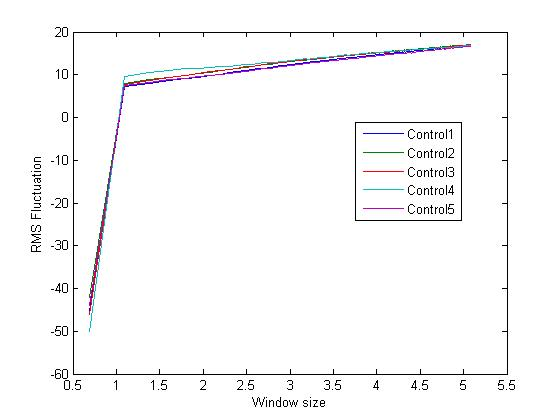
\includegraphics[width=.8\textwidth]{E1.jpg}
\subcaption{DFA result of the control data set}\label{figa}
\endminipage\hfill
\minipage{.5\textwidth}%
\centering
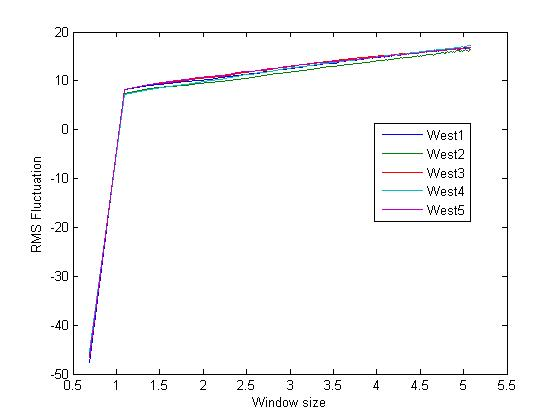
\includegraphics[width=.8\textwidth]{E2.jpg}
\subcaption{DFA result of the west data set}\label{figb}
\endminipage\hfill
\caption{Detrended fluctation analysis plots of the two data set}
\end{figure}


\begin{table}[!htbp]
\centering
\caption{}\label{c1}
\begin{tabular}{ c c c c c c c c} 
\hline
$Control$&$1$&$2$&$3$&$4$&$5$&$\mu$&$\sigma$\\
\hline
$FD $&$1.7438$&$1.7298$&$1.7707$&$1.7208$&$1.7173$&$ 1.7365$&$ 4.7074e-04$\\
$1/f$&$-1.3486$&$-1.0308$&$-1.0754$&$-1.0624$&$-1.5117$&$-1.2058$&$ 0.0455$\\
$LE$&$0.0826$&$0.3860$&$0.2120$&$0.0825$&$0.0944$&$0.1938$&$0.0198$\\
$SampEnResults$&$2.3058$&$2.0164$&$2.0987$&$1.8646$&$2.1077$&$2.0786$&$0.0256$\\
&$0.6178$&$0.6472$&$0.7670$&$0.4271$&$0.5736$&$0.6065$&$0.0152$\\
\hline 
\end{tabular}
\end{table}

\begin{table}[!htbp]
\centering
\caption{}\label{c2}
\begin{tabular}{ c c c c c c c c} 
\hline
$West$&$1$&$2$&$3$&$4$&$5$&$\mu$&$\sigma$\\
\hline
$FD$&$1.7448$&$1.5999$&$1.7198$&$1.7501$&$1.7059$&$ 1.7041$&$ 0.0037$\\
$1/f$&$-1.0898$&$-1.5659$&$-1.0138$&$-1.3829$&$-1.1288$&$-1.2362$&$ 0.0532$\\
$LE$&$0.1217$&$0.0878$&$0.2797$&$0.0807$&$0.3043$&$0.3222$&$0.0829$\\  
$SampEnResults$&$2.0307$&$2.2033$&$2.1825$&$2.1837$&$2.2467$&$2.1694$&$0.0067$\\
&$1.0327$&$0.6303$&$0.8739$&$0.5220$&$0.6609$&$ 0.7440$&$0.0423$\\
\hline 
\end{tabular}
\end{table}

Non linear analysis of heart rate variability (HRV) aims consistent inference the underlying phenomenon associated with the signal. 
The analysis is divided into two main set of the approaches. 

Starting with the scaling behavior of the non-linearity fractal dimension (FD) is capable of evaluating the complexity degree associated with the signal. This is computed via the of velocity that measurement increases of decreases as the scale tends to increases or decreases. Generally speaking, for abnormal subjects the rhythmic variation tends to decreases consequently FD in this case will be lower than normal subjects. Comparing the two data set in the \textbf{\textit{Control}} case in table \ref{c1} the values of the are fairly high, and there is no variation among the entities. In comparison to the \textbf{\textit{West}} the FD values are on average lower. The variation is slightly higher in this case where in addition the second measurement tends to have a significantly lower value implying some anomalies associated with this patient. Statistically speaking, the west data set on average tends to have less rhythmic heart rate table \ref{c2}.

\textbf{1/f} slope is another important characterisation of the HRV. The smoothness of the time series what the slope values claim to indicate. The values of abnormalities tends to be slightly lower compare to normal HR. In the \textbf{\textit{Control}} data set this values on average tend to be lower compare to the \textbf{\textit{West}} data set although the difference is relatively small. Regarding the variation of this value in the \textbf{\textit{West}} dataset it tends to be bigger. In both group of measurements there are some samples with significantly lower value of slope compare to the mean. In the \textbf{\textit{Control}} case the second, third and fourth sample have a fairly small value. Whereas on the \textbf{\textit{West}} data set the first and the third sample has dramatic low value. 

The other set of measurements consist on the chaos complexity of the system. This methods are mainly based on the chaos theory.

Herein the Lyapunov exponent is the first to be explored. Geometrically speaking  its values represent the divergence of respective trajectories from their initial position. Consequently slowly varying HR, LE is small meaning that the intensity of the chaotic system is low as well. \textbf{\textit{Control}} likewise the average is significantly smaller compare to the \textbf{\textit{West}} data set. Variance is not a of an important as compare to mean however the \textbf{\textit{West}} data set samples vary more. 

Moving on to the sample entropy. It measures statistically the complexity and regularity of the time-series. Its values are small when the HRV runs under same abnormalities and theoretically should be big when the HRV is normal. Mean value is however smaller in the \textbf{\textit{Control}} and therefore inferring some abnormalities compare to the \textbf{\textit{West}}.    
  
Regarding DFA results for low window size tends to be higher in the control case tends to be higher than one. On the other hand the Control case it higher than the West set comparing respective individuate and therefore on average. Translated into variability the West case on average has a higher variation compare to the Control set in figure \ref{figa} and \ref{figb}. Further more from the table \ref{a2} and \ref{a1} the slopes are computed from the DFA plots are outlined into the both tables. Speaking about the health, Control set has a higher variability compare to the West which is the main indication of the DFA from higher slope value.  
    
    




\begin{table}[!htbp]
\centering
\caption{Slope of the second part of line in DFA plots}\label{a2}
\begin{tabular}{ c c c c c c c c} 
\hline
&$1$&$2$&$3$&$4$&$5$&$\mu$\\
\hline
$Control$&$31.4300$&$ 4.8353$&$4.8058$&$15.0472$&$21.1844$&$6.9868$\\
$West$&$6.9512$&$ 3.7947$&$0.7843$&$ 0.6201$&$13.9351$&$5.2171$\\
\hline 
\end{tabular}
\end{table}





\begin{table}[!htbp]
\centering
\caption{Slope of the first part of line in DFA plots}\label{a1}
\begin{tabular}{ c c c c c c c c} 
\hline
&$1$&$2$&$3$&$4$&$5$&$\mu$\\
\hline
$Control$&$129.5984$&$123.5662$&$132.5211$&$147.3374$&$127.0359$&$132.0118$\\
$West$&$137.6878$&$132.0872$&$135.5602$&$129.5709$&$135.0323$&$133.9877$\\
\hline 
\end{tabular}
\end{table}



\begin{figure}[!htbp]
\minipage{.5\textwidth}%
\centering
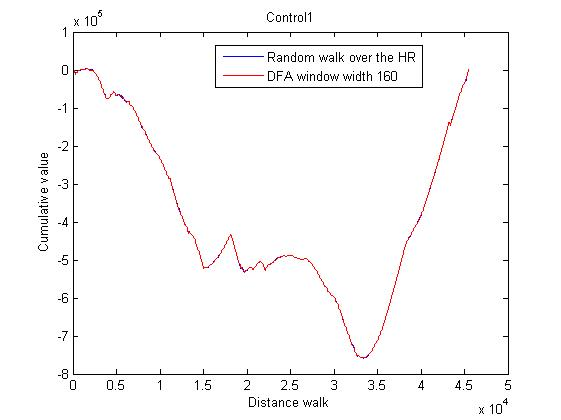
\includegraphics[width=.7\textwidth]{E3.jpg}\\
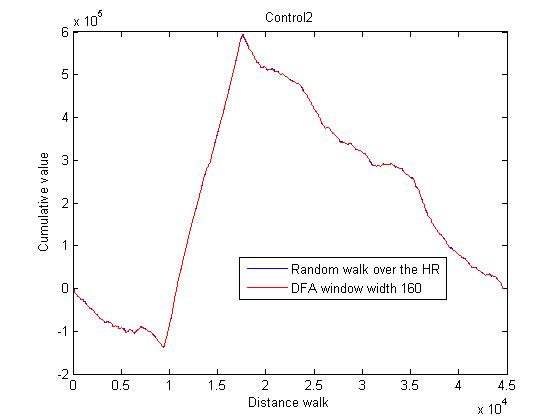
\includegraphics[width=.7\textwidth]{E4.jpg}\\
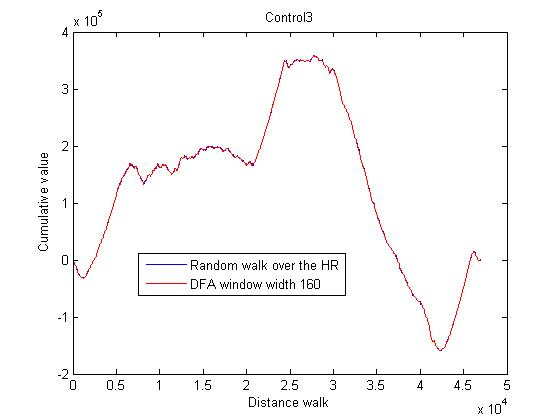
\includegraphics[width=.7\textwidth]{E5.jpg}\\
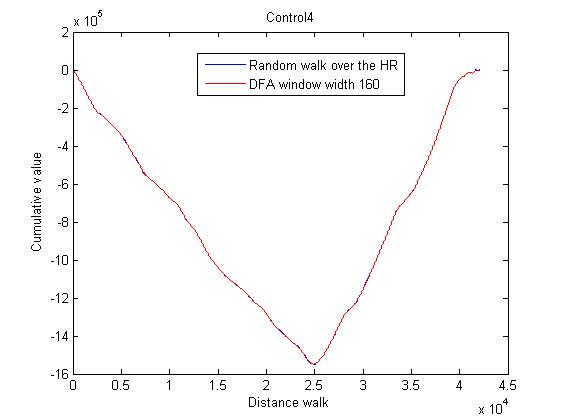
\includegraphics[width=.7\textwidth]{E6.jpg}\\
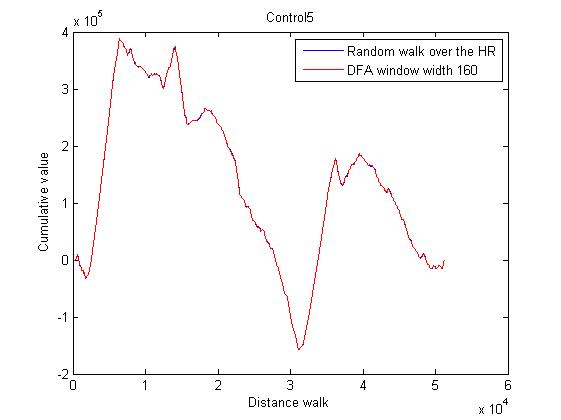
\includegraphics[width=.7\textwidth]{E7.jpg}\\
\subcaption{}
\endminipage\hfill
\minipage{.5\textwidth}%
\centering
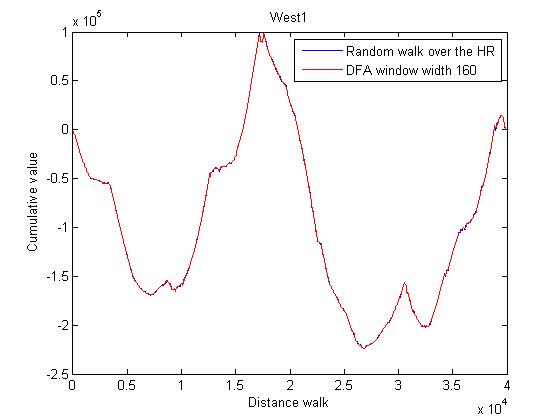
\includegraphics[width=.7\textwidth]{E8.jpg}\\
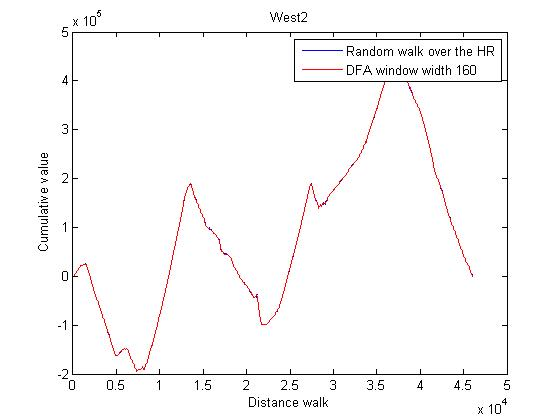
\includegraphics[width=.7\textwidth]{E9.jpg}\\
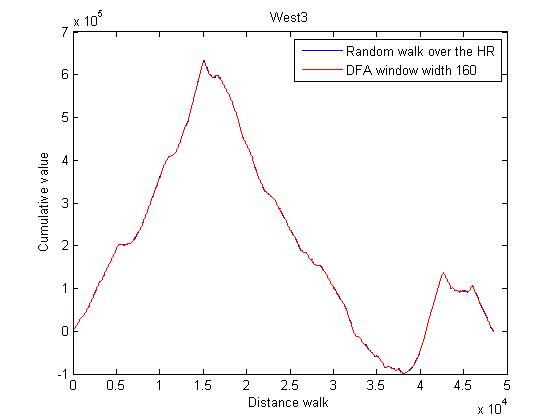
\includegraphics[width=.7\textwidth]{E10.jpg}\\
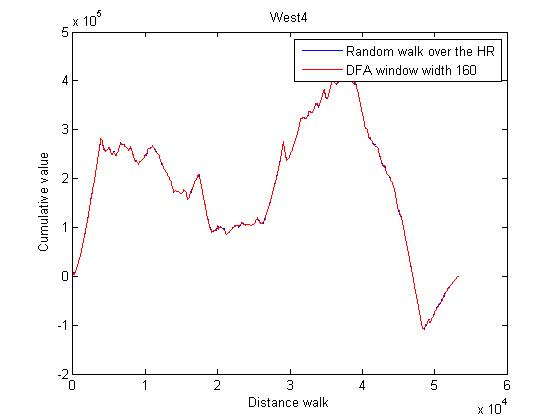
\includegraphics[width=.7\textwidth]{E11.jpg}\\
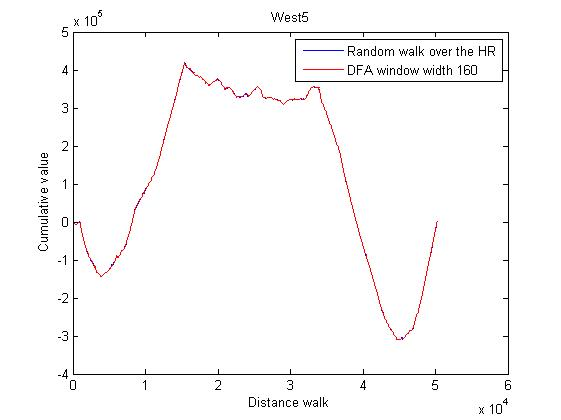
\includegraphics[width=.7\textwidth]{E12.jpg}\\
\subcaption{}
\endminipage\hfill
\caption{DFA result for both of the groups}
\end{figure}










\bibliographystyle{unsrt}
\bibliography{Bibliography}

\clearpage
\appendix

\section{Appendix for question 1}

Signals are uncorrelated if their covariance is zero:

\begin{equation}\label{equati1}
E(y_{1}y_{2})-E(y_{1})E(y_{2})=0
\end{equation}

Signals are independent iff their joined probability is equal the production of the respective probability:

\begin{equation}\label{equati2}
p(y_{1}y_{2})=p(y_{1})p(y_{2})
\end{equation}


Independece implies uncorrelatndess whereas the other way around is not true. 
\section{Additional figure}








\begin{figure}[!htbp]
\minipage{.5\textwidth}%
\centering
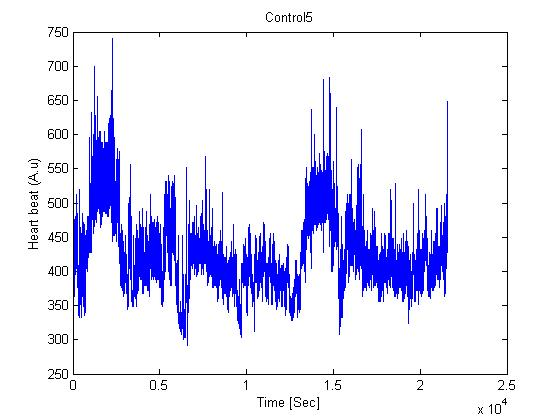
\includegraphics[width=.71\textwidth]{E23.jpg}\\
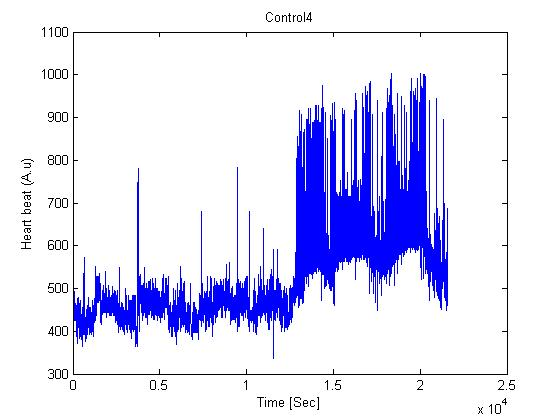
\includegraphics[width=.7\textwidth]{E24.jpg}\\
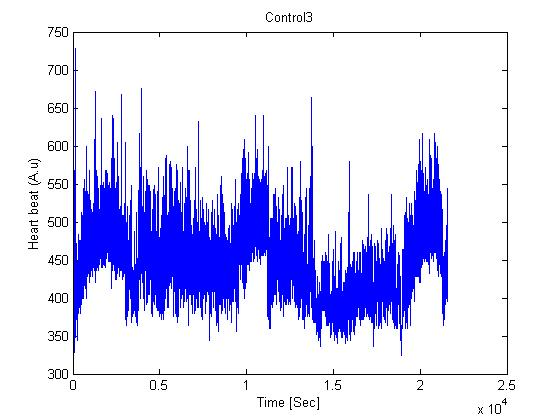
\includegraphics[width=.7\textwidth]{E25.jpg}\\
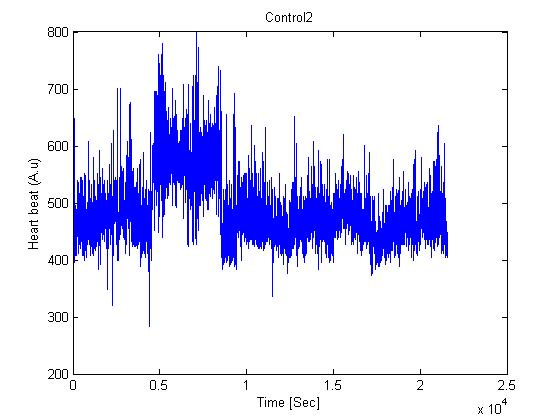
\includegraphics[width=.7\textwidth]{E26.jpg}\\
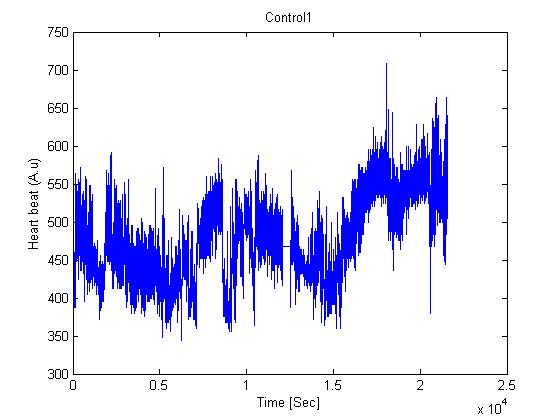
\includegraphics[width=.7\textwidth]{E27.jpg}
\endminipage\hfill
\minipage{.5\textwidth}%
\centering
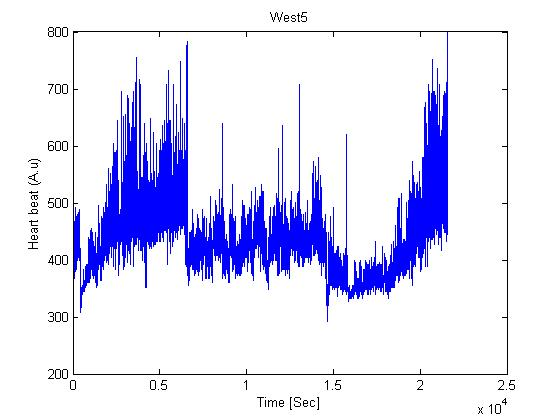
\includegraphics[width=.7\textwidth]{E28.jpg}\\
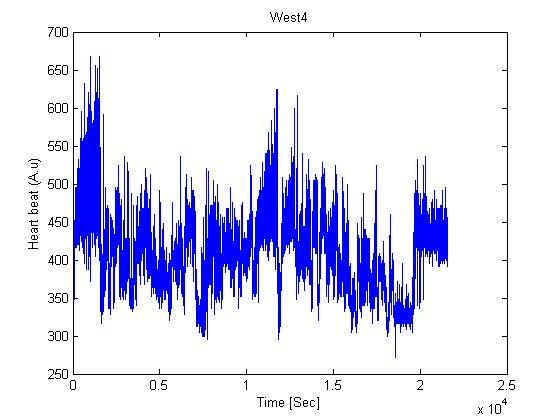
\includegraphics[width=.7\textwidth]{E29.jpg}\\
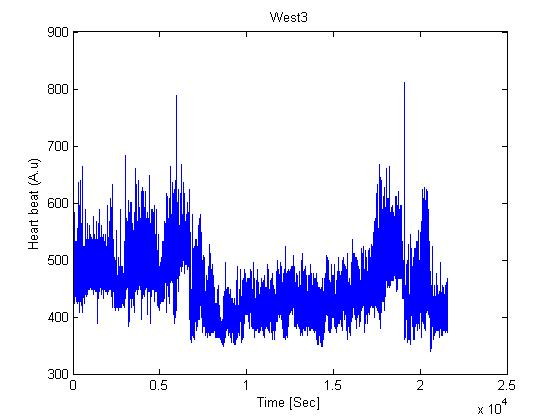
\includegraphics[width=.7\textwidth]{E30.jpg}\\
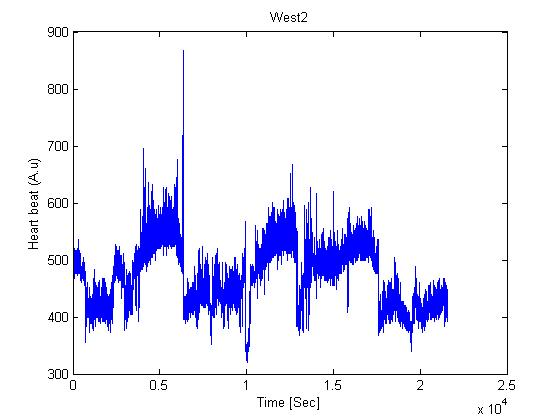
\includegraphics[width=.7\textwidth]{E31.jpg}\\
\includegraphics[width=.7\textwidth]{E32.jpg}
\endminipage\hfill
\caption{Tachogram plots for each measurement}
\end{figure}




\begin{figure}[!htbp]
\minipage{.5\textwidth}%
\centering
\includegraphics[width=.7\textwidth]{E33.jpg}\\
\includegraphics[width=.7\textwidth]{E34.jpg}\\
\includegraphics[width=.7\textwidth]{E35.jpg}\\
\includegraphics[width=.7\textwidth]{E36.jpg}\\
\includegraphics[width=.7\textwidth]{E37.jpg}\\
\subcaption{}
\endminipage\hfill
\minipage{.5\textwidth}%
\centering
\includegraphics[width=.7\textwidth]{E38.jpg}\\
\includegraphics[width=.7\textwidth]{E39.jpg}\\
\includegraphics[width=.7\textwidth]{E40.jpg}\\
\includegraphics[width=.7\textwidth]{E41.jpg}\\
\includegraphics[width=.7\textwidth]{E42.jpg}\\
\subcaption{}
\endminipage\hfill
\caption{F slope fitting}
\end{figure}


\begin{figure}[!htbp]
\minipage{.5\textwidth}%
\centering
\includegraphics[width=.7\textwidth]{E43.jpg}\\
\includegraphics[width=.7\textwidth]{E44.jpg}\\
\includegraphics[width=.7\textwidth]{E45.jpg}\\
\includegraphics[width=.7\textwidth]{E46.jpg}\\
\includegraphics[width=.7\textwidth]{E47.jpg}\\
\subcaption{}
\endminipage\hfill
\minipage{.5\textwidth}%
\centering
\includegraphics[width=.7\textwidth]{E48.jpg}\\
\includegraphics[width=.7\textwidth]{E49.jpg}\\
\includegraphics[width=.7\textwidth]{E50.jpg}\\
\includegraphics[width=.7\textwidth]{E51.jpg}\\
\includegraphics[width=.7\textwidth]{E52.jpg}\\
\subcaption{}
\endminipage\hfill
\caption{Poincare plot}
\end{figure}






\lstset{language=Matlab,%
    %basicstyle=\color{red},
    breaklines=true,%
    morekeywords={matlab2tikz},
    keywordstyle=\color{blue},%
    morekeywords=[2]{1}, keywordstyle=[2]{\color{black}},
    identifierstyle=\color{black},%
    stringstyle=\color{mylilas},
    commentstyle=\color{mygreen},%
    showstringspaces=false,%without this there will be a symbol in the places where there is a space
    numbers=left,%
    numberstyle={\tiny \color{black}},% size of the numbers
    numbersep=9pt, % this defines how far the numbers are from the text
    emph=[1]{for,end,break},emphstyle=[1]\color{red}, %some words to emphasise
    %emph=[2]{word1,word2}, emphstyle=[2]{style},    
}

\newpage
\section{Code for exercise 1}
\lstinputlisting{Main_Exercise_Session_2.m}
\lstinputlisting{Automated_CCA.m}
\lstinputlisting{CCA_Start.m}
\lstinputlisting{Manual_CCA.m}
%\newpage
\lstinputlisting{Poincare.m}
%\newpage
%\lstinputlisting{ccaqr.m}


\newpage
\subsection{Code for exercise 2}
\lstinputlisting{Main_Exercise_Session_2_2.m}
\subsection{Aid function}
\lstinputlisting{DFA.m}
\lstinputlisting{FindSlope.m}
\lstinputlisting{Poincare.m}
\lstinputlisting{F_slope.m}
\lstinputlisting{WindowingFunction.m}
\lstinputlisting{IntegrateRR.m}
\lstinputlisting{LinearLeastSquareOfWindow.m}




\end{document}

